\documentclass[../article.tex]{subfiles}

\usepackage[english]{babel}
\usepackage{amsmath}
\usepackage{graphicx}
\usepackage{wrapfig}
\usepackage[superscript,biblabel]{cite}
\DeclareMathOperator*{\E}{\mathbb{E}}
\DeclareMathOperator*{\argmin}{arg\,min}
\DeclareMathOperator*{\argmax}{arg\,max}

\usepackage[
backend=biber,
style=alphabetic,
citestyle=authoryear
]{biblatex}

\addbibresource{./bib/moosavidezfooli.bib} %Imports bibliography file

\graphicspath{ {./fig/} }

\begin{document}

The main algorithm that I researched for this report was DeepFool, which is an optimized attack method on data for deep neural network classifiers. This technique was first proposed by Moosavi-Dezfooli et al. in their paper, \emph{DeepFool: a simple and accurate method to fool deep neural networks} (moosavidezfooli.bib). The primary attack vector of DeepFool is to introduce instability into a classifier through adversarial perturbations, where minor changes are made to data samples that result in a classifier giving an incorrect output. What distinguishes DeepFool, however, is that it optimizes its attack to have the minimal amount of perturbations applied to the sample data that still tricks a classifier.

\begin{wrapfigure}{r}{0.25\textwidth} %this figure will be at the right
	\centering
	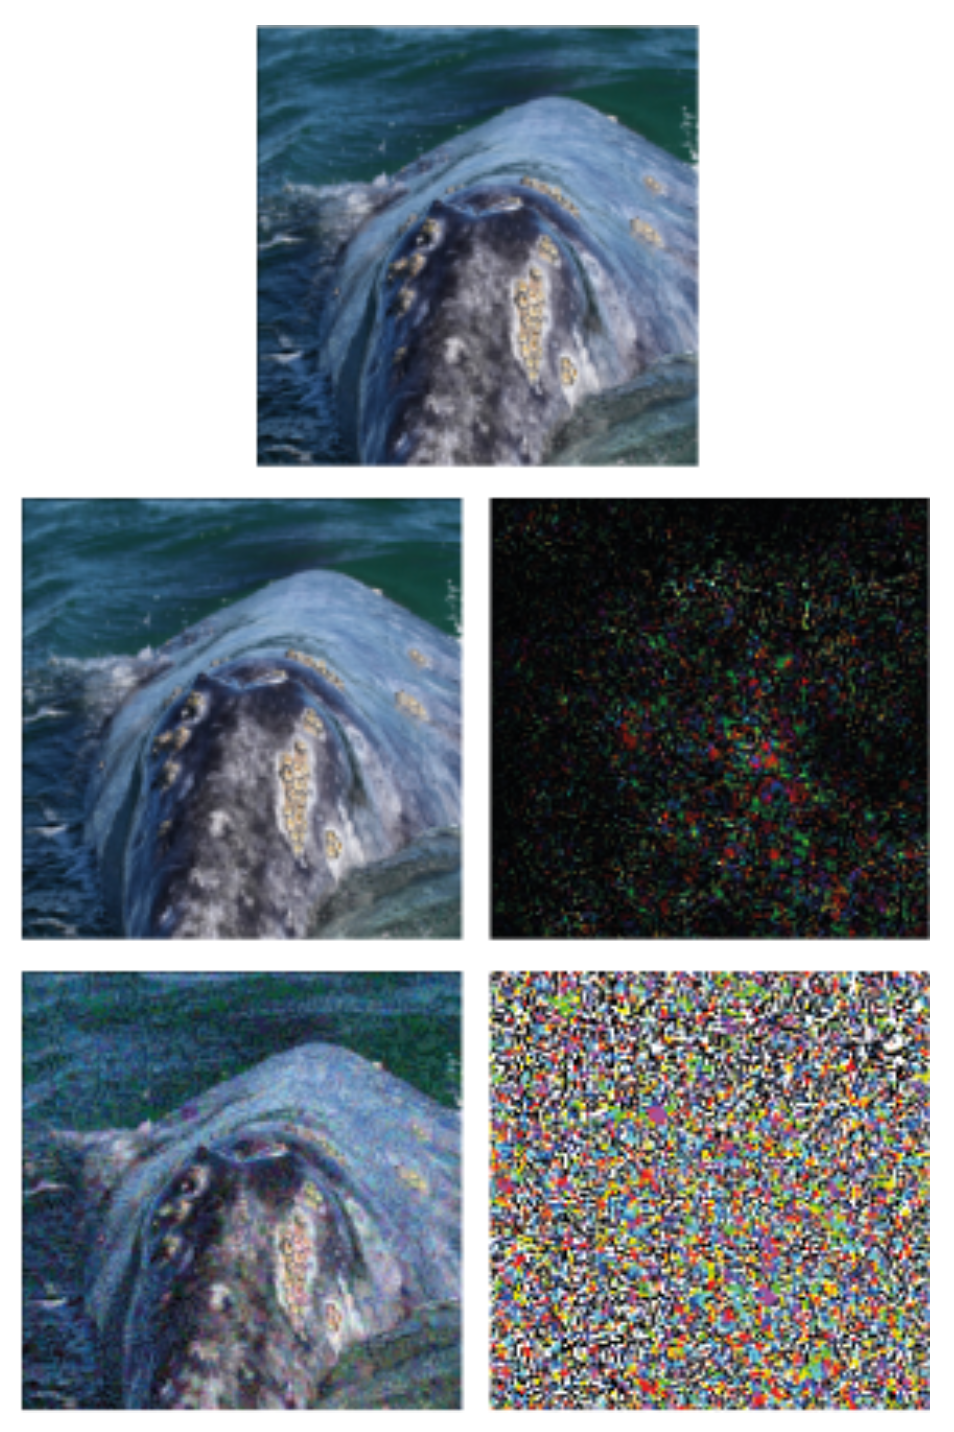
\includegraphics[width=0.25\textwidth]{adv_pert_img.png}
	\caption{\label{fig:Figure 1}Base image (top row). Image perturbed and perturbations by DeepFool (middle row). Image perturbed and perturbations by fast gradient sign method (bottom row).}
\end{wrapfigure}

Adversarial perturbation has seen extensive research outside of DeepFool. First thoroughly explored by Szegedy et al. in 2014, existing research aims to approximate the minimum number of perturbations required to fool a deep neural network classifier (szegedy.bib). However, their optimization method does not scale to larger datasets. These techniques are often overly-expensive in terms of computation, such as the method Nyugen et al. developed to render a data sample unrecognizable to a human, but convince a classifier to classify it with confidence (nyugen.bib). Other researchers created a fast gradient step method (goodfellow.bib), which quickly calculate approximately optimal perturbations, but this estimation can be considerably different from a more optimal solution. Figure 1 demonstrates the perturbations created by DeepFool and those created by the previously-mentioned 'fast gradient step' method. The image was originally classified as a whale, and the noise maps in the right column are the perturbations applied to that image in order for the classifier to declare the augmented image as a turtle instead. It can be clearly observed that DeepFool's perturbations are more minimal in quantity and in their affect on the base image, and was able to achieve the same desired misclassification as the gradient step method.

DeepFool's optimized approach to finding the minimal quantity of perturbations stems from the concept of what a perturbation is. First, they defined an adversarial perturbation as the smallest alteration \textit{\textbf{r}} that can change a classifier's estimated label $\hat{k}(x)$ to be the following (ST means "subject to"):

\[\delta(x:\hat{k}) := \min_r||r||_2  ST \hat{k}(x + r) \neq \hat{k}\]

So, let there be some $\hat{k} = sign(f(x))$, where $f(x)$ is an affine, arbitrary, scalar classification function. The robustness of this classifier, or how resistant it is to error, can be expressed as:

\[ \rho_{adversarial} (\hat{k}) = \mathbb{E}_x \frac{\delta(x:\hat{k})}{||x||_2}\]

Here, $\mathbb{E}_x$ represents the expectation over the distribution of all data. With these two expressions, the researchers determined that, as an affine classifier, the distances between points on the classifier's affine hyperplane $w^T x + b = 0$ and its robustness could be determined, and subsequently, so too could the minimum number of perturbations required to cross that threshold. When computed linearly, they derived the expression for that minimum number of permutations as:

\[r_*(x_0) := \argmin ||r||_2 ST sign(f(x_0+r)) \neq sign(f(x_0)) = -\frac{f(x_0)}{||w||_2^2 w}\]

\[\argmin_{r_i} || r_i ||_2 ST f(x_i) + \nabla f(x_i)^T r_i = 0\]

Perturbation $r$ at index $i$ is computed, and then the next $x_{i+1}$ is updated. This continues until the classifier estimator $\hat{k}$ changes, and thus the prediction changes to the intended wrong label.

\begin{wrapfigure}{l}{0.4\textwidth} %this figure will be at the right
	\centering
	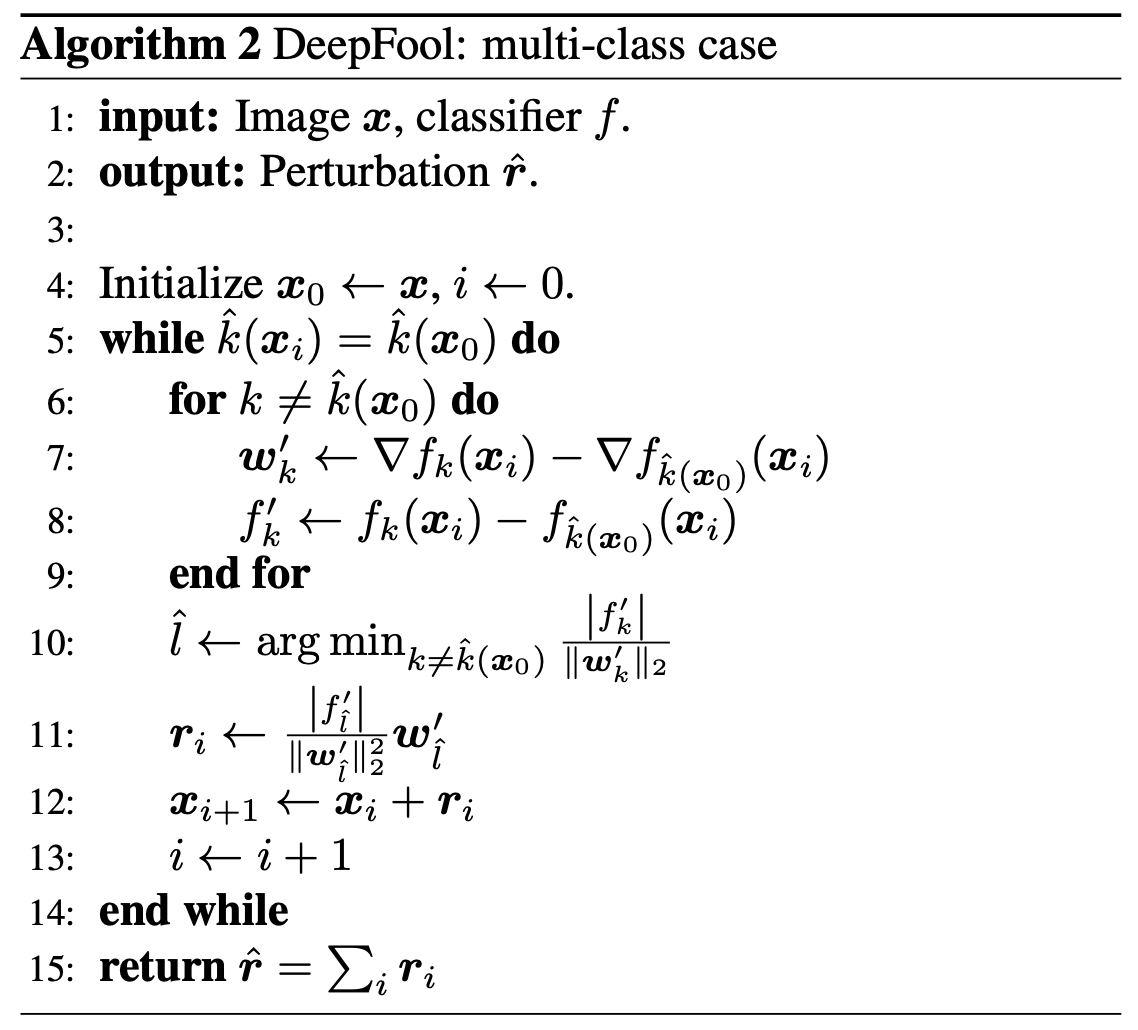
\includegraphics[width=0.4\textwidth]{deepfool_multi_class.png}
	\caption{\label{fig:Figure 2}Pseudocode of the mutliclass iteration of the DeepFool adversarial perturbation attack.}
\end{wrapfigure}

The DeepFool adversarial perturbation optimization method was then expanded to cover mutliclass problem spaces. The researchers treated multi-class classification as an aggregation of binary classification problems, of which the best option is selected. They represent this as, for a classification estimator, $\hat{k}(x) = \argmax_{k} f_k(x)$, where it iterates over each $k$ class. For an affine classifier in this case, an arbitrary classification function can be defined as $f(x) = W^Tx + b$, and the minimum amount of perturbations necessary to change its result is:

\[\argmin_{r} ||r||_2 s.t. \exists k: w_k^T(x_0 + r) + b_k \geq w_{\hat{k}(x_0)}^T (x_0+r) + b_{\hat{k}(x_0)}\] 

This equality is similar in terms of geometric distance to that of the distance between some point, $x_0$, and the complement of a polyhedron $P$ that contains it. In this situation, polyhedron $P$ represents the geometric space equivalent to the classification estimator output $\hat{k}(x_0)$. This problem was solved for with binary classification, however, and that solution can be modified to cover this problem. By letting $\hat{l}(x_0)$ represent the nearest hyperplane to the boundary of polyhedron $P$, the minimum amount of perturbations can then be calculated as a vector that projects the label onto that hyperplane. The final implementation of this derivation can be seen in Figure 2, which depicts the full mutliclass algorithm for DeepFool.

The second algorithm that I researched, One Pixel Attack from Vargas et al.'s paper \emph{One Pixel Attack for Fooling Deep Neural Networks}, approched the same concept as DeepFool, but from a much different perspective (vargas.bib). While the DeepFool attack method would optimize how many perturbations it needs to an image in order to deceive a classifier, One Pixel Attack aims to determine a single pixel in an image that, when changed, would most likely fool the classifier. Additionally, the One Pixel Attack is a semi-black-box attack, where the only data it needs from the classifier are the output probability labels. This stands in contrast to the DeepFool attack, which needed access to the classifiers internal functions to best counter them. By operating as more of a black-box, where the internal mechanisms of the underlying classifier remain hidden, the One Pixel Attack becomes more versatile, as those data points are easier to access.

As the amount of information available to the One Pixel Attack is limited to its assumptions about the input data and the existing probability labels. Vargas et al. begin with the problem that for an $n-dimensional$ input, the flattened array of pixels $x$ is the original image that would be properly classified. They then propose that the probability of that input image belonging to an arbitrary class $k$ be $f_k(x)$. From here, the researchers create a new $n-dimensional$ vector, which holds adversarial perturbations that are defined by:

\[\max_{e(x)^*} f_{a}(x + e(x)) ST ||e(x)||_0 \leq d\]

In this maximizing expression, the perturbations are defined by the original image $x$, the target class $a$, and the small number limit $d$ to which the value can be modified. Only a subset of size $d$ dimensions are being modified, and the unaffected perturbations in the new vector $e$ are left to be zero. In essence, this allows the One Pixel Attack to radically perturb a small, but significant, portion of the input image. These narrow sections are refined by a differential evolution (DE) algorithm, which is a population-based optimization method for multi-part problems. As it does not utilize a gradient to theorize about an optimal solution, the DE algorithm does not need to know about the classifier's internal objective functions. Instead, it can independently iterate through generations of candidates before reaching what it considers to be most optimal.

I implemented the DeepFool and One Pixel Attack algorithms, along with a custom extension of DeepFool called Dynamic DeepFool. The authors of the DeepFool paper, Moosavi-Dezfooli et al., noted that their iteration towards a class boundary was always multiplied by a small constant, $\eta$. Furthermore, in my research I came across experiments where several DeepFool attackers

\begin{figure}[H]
	\begin{tabular} {|p{2cm}|p{2cm}||p{2cm}|p{2cm}|p{2cm}|p{2cm}|p{1.5cm}|}
		\hline
		Attack & DataSet  & Accuracy & Precision & Recall & AUC & Loss\\
		\hline
		\hline
		DeepFool & MNIST & 99.3 & 0.993 & 0.993 & 0.997 & 0.0647 \\
		\hline
		DeepFool & CFAIR-10 & 0.78.7 & 0.846 & 0.739 & 0.976 & 0.620 \\
		\hline
		Dynamic DeepFool & CFAIR-10 & 81.4& 0.864 & 0.766 & 0.980 & 0.549 \\
		\hline
		One Pixel Attack & CFAIR-10 & 59.4 & 0.688 & 0.478 & 0.919 & 1.214 \\
		\hline
	\end{tabular}
	\caption{Initial results of classifiers before attacks were applied (control group).}
	\label{fig:ep0.3}
\end{figure}

\begin{figure}[H]
	\begin{tabular}{ |p{2cm}|p{2cm}||p{1.5cm}|p{1.5cm}|p{1.5cm}|p{1.5cm}|p{1.5cm}|p{1.5cm}|}
		\hline
		Attack & DataSet  & \% Success Rate & Adv Accuracy & Precision & Recall & AUC & Loss\\
		\hline
		\hline
		DeepFool & MNIST & 8.70 & 92.3 & 0.923 &0.922 & 0.967 & 0.9035 \\
		\hline
		DeepFool & CFAIR-10 & 87.60 & 19.20 & 0.0563 & 0.03 & 0.746 & 3.783  \\
		\hline
		DeepFool & CFAIR-10 & 90.20 & 15.20 & 0.067 & 0.044 & 0.707 & 5.021 \\
		\hline
		DeepFool & CFAIR-10 & 92.60 & 14.80 & 0.0937 & 0.066 & 0.688 & 5.257 \\
		\hline
		\hline
		Dynamic DeepFool & CFAIR-10 & 97.60 & 12.20 & 0.060 & 0.034 & 0.730 & 3.938 \\
		\hline
		Dynamic DeepFool & CFAIR-10 & 98.60 & 11.60 & 0.072 & 0.052 & 0.690 & 5.571 \\
		\hline
		Dynamic DeepFool & CFAIR-10 & 98.40 & 13.40 & 0.063 & 0.042 & 0.709 & 4.564 \\
		\hline
		One Pixel Attack & CFAIR-10 & 19.80 & 43.6 & 0.436 & 0.436 & 0.690 & 8.856\\
		\hline
		One Pixel Attack & CFAIR-10 & 18.80 & 35.8 & 0.358 & 0.358 & 0.646 & 10.159\\
		\hline
	\end{tabular}
	\caption{Results of attacks on designated datasets. Attacks with MNIST were performed with default Keras classifier. Attacks with CFAIR-10 were performed with custom Keras classifier, as shown in Figure 5.}
	\label{fig:ep0.4}
\end{figure}

\begin{wrapfigure}{l}{0.4\textwidth} %this figure will be at the right
	\centering
	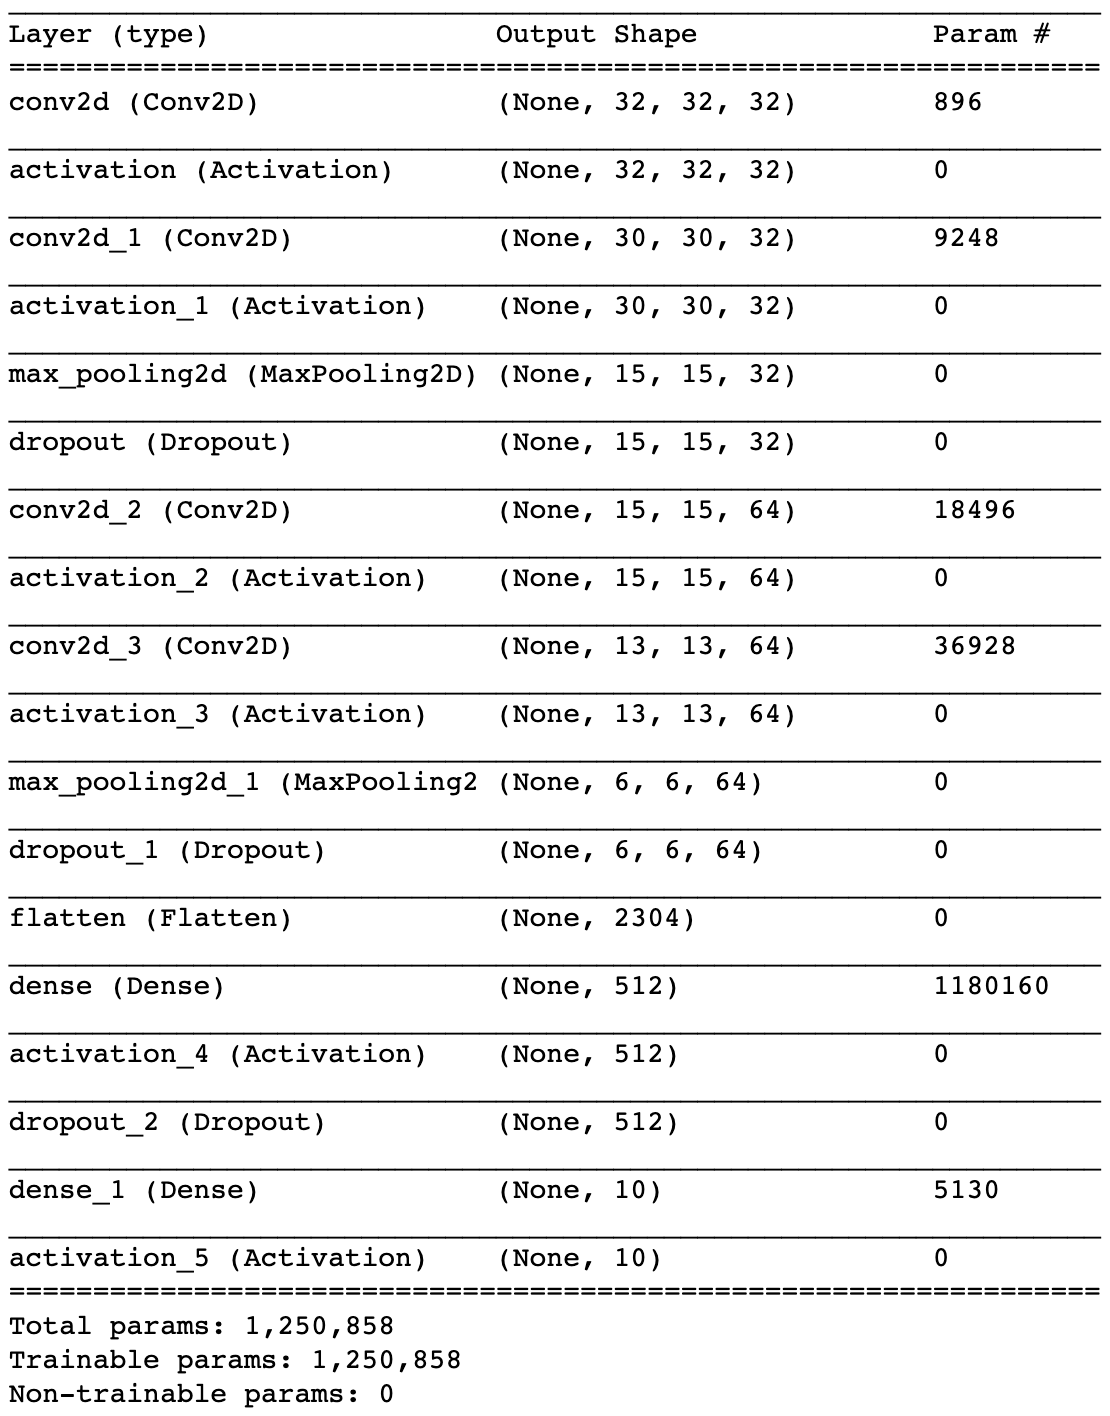
\includegraphics[width=0.4\textwidth]{cnn_arch.png}
	\caption{\label{fig:Figure 5} Architecture of deep neural network used in CFAIR-10 tests.}
\end{wrapfigure}

\noindent were trained in tandem, with the only difference being their $\eta$ value. So, utilizing a principle of gradient descent, I created a version of DeepFool that possessed a dynamical $\eta$ value. The value of the learning constant $\eta$ was determined by the following expression: $0.0001 * \log(i + 2)$, where $i$ was the current iteration count. Instead of the default value of $10e^6$, $\eta$ would begin larger and rapidly approach its target value. Then, its step size would begin to decrease as it approached.

The DeepFool algorithm was tested on both the MNIST and CFAIR-10 datasets, while the Dynamic DeepFool and One Pixel Attack methods were only tested on the CFAIR-10 dataset, which allows for a more direct comparison. From the same deep convolutional neural network architecture depicted in Figure 5, three classifiers were generated for each CFAIR-10 test. Before any attack was tested, each model was fitted, and their initial average performance is shown in Figure 3. The results shown in Figure 4 state the respective model's performance on adversarially-generated test samples, but their training data remained unmodified. The "\% Success Rate" column in Figure 4 denotes the percentage of provided adversarial samples that successfully fooled the classifier.

With regards to the MNIST dataset, while there was a noticeable decrease in accuracy, precision, recall, and AUC (as well as an increase in loss), the size of that decrease was inconsistent with all of the CFAIR-10 results, and it remains unclear how consistent it is with the original researchers. Moosavi-Dezfooli et al.'s original paper was not concerned with the direct performance metrics of the models which suffered a DeepFool attack, but rather the quantity of perturbations and general robustness of already established algorithms. Thus, there is no comparable data to contrast this anomaly with. 

With regards to the performance difference between the DeepFool (DF1) and Dynamic DeepFool (DF2), the results demonstrated potential for further refinement. While each algorithm was largely successful in their attack on the classifier, DF2 outperformed DF1 in each recorded metric. DF2 caused, on average, a greater rate of misclassification than DF1 did. An additional difference that may warrant further analysis is the difference in time between DF1 and DF2 to complete an attack. If DF2 can reach its boundary faster than DF1, that will result in the conservation of computational resources.

With regards to the One Pixel Attack algorithm, this implementation's results are consistent with those of the original authors. Vargas et al. recorded a decrease in accuracy by 16.89\%, from 85.6\% to 68.71\% after a non-targeted, one-pixel attack. This implementation caused the associated classifier to drop its accuracy by, on average, 19.7\%. Considering that the initial accuracy wasn't as high as that recorded in Vargas et. al, it is likely that this instance's provided classifier was not as strong, and thus more prone to failure. Nevertheless, these results do appear to reconcile with the established literature.



\printbibliography

\end{document}